\documentclass{beamer}

\usepackage{amssymb}
\usepackage[english]{babel}
\usepackage{graphicx}
\usepackage{physics}
\usepackage{siunitx}

\usetheme{Berlin}
\usecolortheme{beaver}
\setbeamertemplate{footline}[frame number]
\graphicspath{ {./img/} }

\title{MCMC of 2D CDT}
\author{T.B.H. Gerstel \and J.G.R. van der Duin}
\date{December 2021}
\institute{Radboud University Nijmegen}
\logo{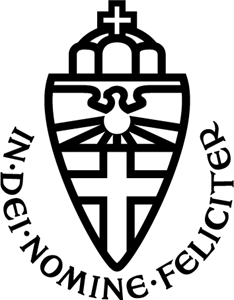
\includegraphics[height=1cm]{radboud}}

\begin{document}

\frame{\titlepage}

\begin{frame}
    \frametitle{Overview}
    \tableofcontents
\end{frame}

\section{Introduction}

\begin{frame}
    \frametitle{Goal}
    Extract information from Quantum Gravity path integral:
    \begin{equation}
        Z = \int \mathcal{D}[g_{\mu \nu}] e^{i S[g_{\mu \nu}]}
    \end{equation}
    With Einstein-Hilbert action:
    \begin{equation}
        S[g_{\mu \nu}]
        =
        \frac{1}{16 \pi G}
        \int_\mathcal{M} \dd[4]{x} \sqrt{-g}
        (R(x) - 2 \Lambda)
    \end{equation}
    Extracting observables:
    \begin{equation}
        \ev{\mathcal{O}}
        =
        \frac{1}{Z} \int \mathcal{D}[g_{\mu \nu}]
        \mathcal{O}[g_{\mu \nu}]
        e^{i S[g_{\mu \nu}]}
    \end{equation}
\end{frame}

\section{Theory}

\begin{frame}
    \frametitle{Causal Dynamical Triangulations}
    How do we sum over all geometries? \\
    Use dynamical triangulations! \\
    But we can do better: Incorporate causal structure in triangulation \\
    Foliate $d$-dimensional triangulation into $(d - 1)$-dimensional slices \\
    %TODO plaatje van een CDT
\end{frame}

\begin{frame}
    \frametitle{Technicalities}
    Restrict to $1 + 1D$: curvature term is constant (Gau\ss -Bonnet) \\
    \begin{equation}
        S[T] \propto \text{Vol}(T) \propto N_2(T)
    \end{equation}
    After Wick rotation:
    \begin{equation}
        Z = \sum_{T} \frac{1}{C_T} e^{-\lambda N_2(T)}
    \end{equation}
    Label the triangles to simplify symmetry
    \begin{equation}
        Z_\ell = \sum _{T_\ell} \frac{1}{N_2(T_\ell)!} e^{-\lambda N_2(T)}
    \end{equation}
\end{frame}

\section{MCMC algorithm}

\begin{frame}
    \frametitle{Volume fixing}
    Split $Z$ into fixed volume contributions:
    \begin{equation}
        Z
        =
        \sum_{T_\ell} \frac{1}{N_2(T_\ell)!} e^{-\lambda N_2(T_\ell)}
        =
        \sum_{n = 0}^\infty \Omega(n) \frac{e^{-\lambda n}}{n!}
    \end{equation}
    It turns out that $\Omega(n) \sim n! 2^n$ \\
    Problem:
    \begin{itemize}
        \item $\lambda > \ln 2$: typical triangulation has a very small volume $\to$ cannot extract useful data
        \item $\lambda < \ln 2$: triangulation keeps growing $\to$ equilibrium cannot be reached
    \end{itemize}
    Our solution: fix the number of triangles $N_2$ \\
    Futher advantage: distribution becomes uniform
\end{frame}

\begin{frame}
    \frametitle{Volume fixing (2)}
    How can we implement this volume fixing? \\
    Possible solution: add a constraint term $\delta S = \epsilon \abs{N_2(T) - n}$ \\
    Issues:
    \begin{itemize}
        \item Introduces an extra parameter $\epsilon$
        \item Results in more rejections
    \end{itemize}
    Our solution: use update rules that preserve $N_2$
\end{frame}



\end{document}